\chapter{Nanowire Structure and Measurement}
\section{Brief Description of Nanowire Structure}
The nanowire we use is made by Prof.Yang's team (National Chiao Tong University)\cite{C5}.
A sectional view of the nanowire structure is given below.
The fabrication process is based on the poly-silicon sidewall spacer technique.
The n-Type doped poly-SiNW FET has 2 to 10 poly-silicon channels.
Each channel is 80nm in width and 2µm in length.
Large portion of the channel surface is exposed to environment.
The exposed region, through several post-process, capture the DNA probe and serve as the sensing site for DNA molecules.\cite{C5, C6}

\begin{figure}[!htbp]
    \centering
    {\fontfamily{pag}\selectfont\textbf{
        \def\svgwidth{5.0cm}
        \fontsize{6}{7}\selectfont
        \input {images/drawing.pdf_tex}
    }}
    \fontsize{6}{7}\selectfont
    \caption{Nanowire Structure}
    \label{fig:drawing}
\end{figure}



\section{Measurement}
This section presents the results.

\subsection*{Front Gate and Back Gate}
Two gates are available: floating gate (liquid gate) and back-gate.
We choose floating gate as the operation gate in spite of some advantages that back-gate has.
One of them is the ability to lower the 1/f noise \cite{C7, C8}.
However, this only happens in a very high gate voltage, which is not practical in the integrated circuit design.
Moreover, the floating gate induces larger drain-current.
In other words, it has higher transconductance. And a high transconductance leads to a stronger feedback ability in our design.

% \begin{figure}[!htbp]
%     \centering
%     {\fontfamily{pag}\selectfont\textbf{
%         \def\svgwidth{5.0cm}
%         \fontsize{6}{7}\selectfont
%         \input {images/FgBg_Compare_Id_dev.pdf_tex}
%     }}
%     \fontsize{6}{7}\selectfont
%     \caption{}
%     \label{fig:res}
% \end{figure}
%
% \begin{figure}[!htbp]
%     \centering
%     {\fontfamily{pag}\selectfont\textbf{
%         \def\svgwidth{5.0cm}
%         \fontsize{6}{7}\selectfont
%         \input {images/FgBg_Compare_Id.pdf_tex}
%     }}
%     \fontsize{6}{7}\selectfont
%     \caption{}
%     \label{fig:res}
% \end{figure}


\begin{figure}[!htbp]
    \centering
    \begin{minipage}[t][0.1\textheight]{1\textwidth}
        \centering
        \def\svgwidth{10cm}
        \fontsize{6}{15}\selectfont
        \input {images/FgBg_Compare_Id.pdf_tex}
        (a)
    \end{minipage}
    \vfill
    \begin{minipage}[t][0.1\textheight]{1\textwidth}
        \centering
        \def\svgwidth{10cm}
        \fontsize{6}{15}\selectfont
        \input {images/FgBg_Compare_Id_dev.pdf_tex}
        (b)
    \end{minipage}
    \caption{}
    \label{fig:IdVgandgbsId}
\end{figure}

\subsection{Parameters}
The most crucial parameter for our circuit design is the transconductance (gm).
{\color{red}
    The gm is acquired by finding the relation between drain-to-source current ($I_d$) and gate-source voltage ($V_g$), and perform differentiation: $\frac{\partial I_d}{\partial V_g}$.
    use standard PBS as
}

\begin{figure}[!htbp]
    \centering
    \begin{minipage}[t][0.1\textheight]{1\textwidth}
        \centering
        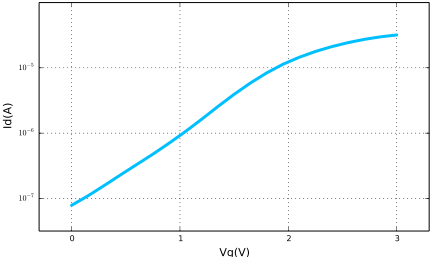
\includegraphics[width=0.6\textwidth,natwidth=610,natheight=442]{images/pIdVg.png}
        (a)
    \end{minipage}
    \hfill
    \begin{minipage}[t][0.1\textheight]{1\textwidth}
        \centering
        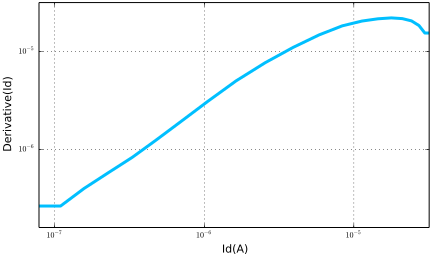
\includegraphics[width=0.6\textwidth,natwidth=610,natheight=442]{images/pIdgbs.png}
        (b)
    \end{minipage}
    \caption{}
    \label{fig:pIdVg}
\end{figure}

The Id-Derivative figures indicates there is a ``linear region'' where gm is proportional to Id.
This property implies the transconductance can be controlled in simple way.
As mentioned in introduction, we may find specific bias Id for distinct elements and adjust their transconductance to a same value.



We also prove that the transconductance under this region is unaffected by the drain-source voltage variance.

\begin{figure}[!htbp]
    \centering
    % {\fontfamily{pag}\selectfont\textbf{
        % \def\svgwidth{10cm}
        % \fontsize{6}{10}\selectfont
        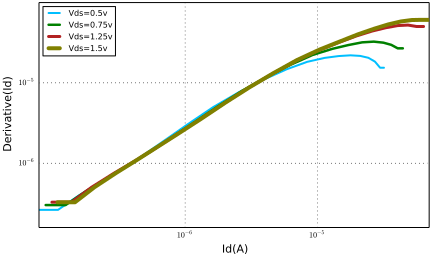
\includegraphics[width=0.8\textwidth,natwidth=610,natheight=642]{images/pIdgbs_Vd.png}
    % }}
    \fontsize{6}{10}\selectfont
    \caption{Id-transconductance with Vds variance}
    \label{fig:Idgbs_Vd}
\end{figure}




\begin{figure}[!htbp]
    \centering
    % {\fontfamily{pag}\selectfont\textbf{
    \def\svgwidth{10cm}
    \fontsize{6}{10}\selectfont
    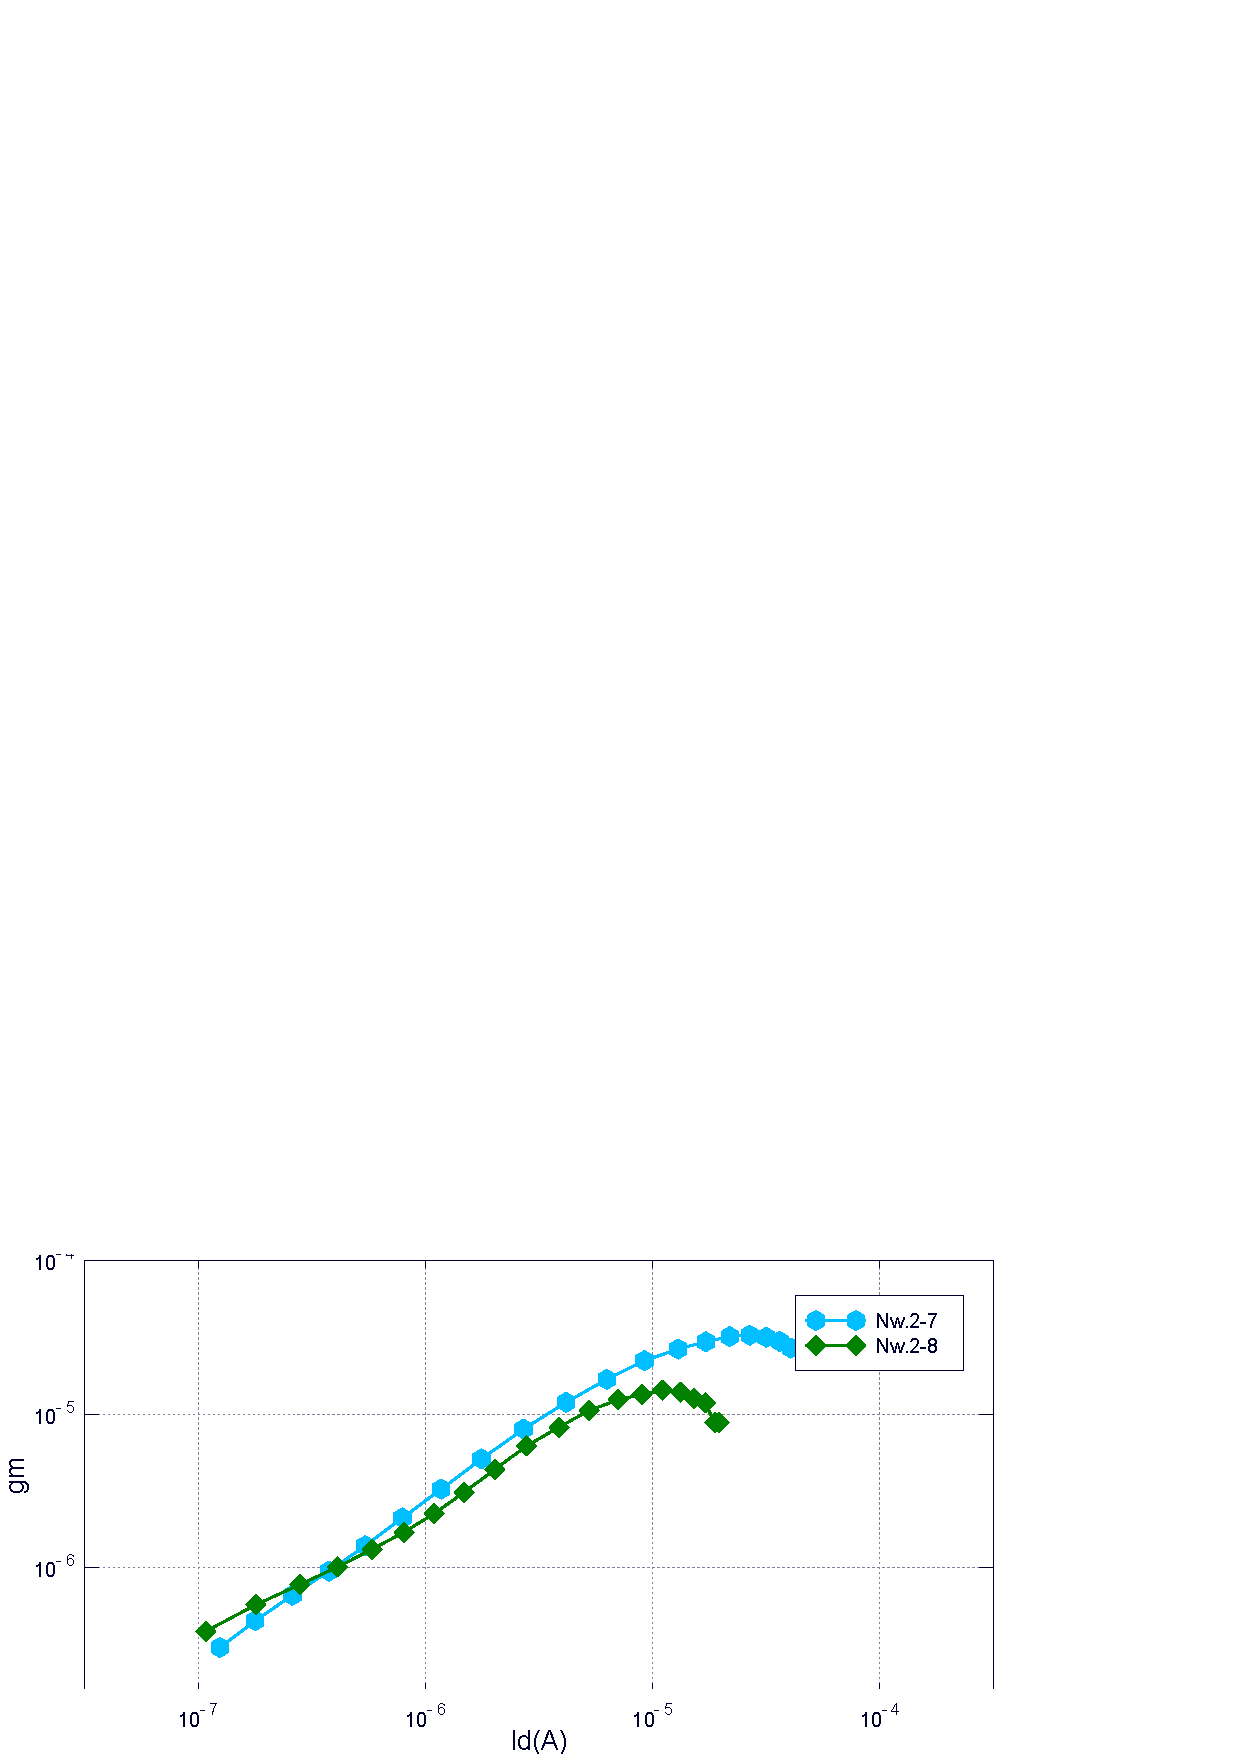
\includegraphics[width=0.8\textwidth,natwidth=610,natheight=642] {images/pDisparity.png}
    % }}
    \fontsize{6}{10}\selectfont
    \caption{Distinct element with a line idicate they have same transconductance}
    \label{fig:disparity}
\end{figure}
By measuring two nanowire element which lie on the same wafer and are immersed with the same testing PBS solution









 

